% \PassOptionsToPackage{subsection=false}{beamerouterthememiniframes}
\documentclass{beamer}
\usepackage[utf8]{inputenc}
\usepackage[english]{babel}
\usepackage{beamerthemeshadow}
\usepackage{xcolor}
\usepackage{booktabs}
\usepackage{tabto}
\usepackage{multirow}
\usepackage[beamer]{hf-tikz}
% \setbeameroption{show notes on second screen=right}

\setbeamertemplate{navigation symbols}{}
\usetheme{Szeged}

\definecolor{userColor}{rgb}{0.06640, 0.5390, 0.2304}
\usecolortheme[named=userColor]{structure}

\beamersetuncovermixins{\opaqueness<1>{25}}{\opaqueness<2->{15}}

\newcommand{\sinc}{{\bf s{\i}nc}({$i$})}
\newcommand{\highlight}[1]{\colorbox{blue!50}{$\displaystyle#1$}}
\renewcommand{\thefootnote}{\alph{footnote}}

\title{MicroRNA prediction from genome-wide data with deep learning: a novel approach based on convolutional residual networks}
\author[Cristian Yones]{C. Yones, L.A. Bugnon, J. Raad, D.H. Milone and G. Stegmayer}
\institute[\sinc - CONICET]{Research Institute for Signals, Systems and Computational Intelligence}
\date{November 13, 2019}

\makeatletter
\setbeamertemplate{footline}
{
  \leavevmode
  \hbox{
    \begin{beamercolorbox}[wd=.5\paperwidth,ht=2.25ex,dp=1ex,center]{author in head/foot}
      \usebeamerfont{author in head/foot}\insertshortauthor~\insertshortinstitute~\beamer@ifempty{\insertshortauthor}{}{}
    \end{beamercolorbox}
  }
  \begin{beamercolorbox}[wd=.5\paperwidth,ht=2.25ex,dp=1ex,center]{date in head/foot}
    \usebeamerfont{date in head/foot}\insertshortdate{}\hspace*{2em}
    \insertframenumber{} / \inserttotalframenumber\hspace*{2ex}
  \end{beamercolorbox}
  \vskip0pt
}

\setbeamertemplate{title page}
{
  \setbeamercolor{lowcol}{fg=white,bg=userColor}

  \begin{centering}

    \begin{columns}
      \begin{column}{0.15\textwidth}
	
\includegraphics[width=\textwidth]{./res/logo.pdf}
      \end{column}
      \begin{column}{0.85\textwidth}
	\begin{minipage}{\textwidth}
	  \usebeamerfont{institute} \scriptsize X Argentinian Conference on Bioinformatics and Computational Biology \\
	  \tiny \insertdate
	\end{minipage}
      \end{column}
    \end{columns}

    \vfill
    \vspace{10pt}

    \begin{beamerboxesrounded}[lower=lowcol,shadow=true]{}
      \centering \usebeamerfont{title}\inserttitle
    \end{beamerboxesrounded}

    \vspace{5pt}

    \usebeamerfont{author}\insertauthor

    \vspace{5pt}

    \usebeamerfont{institute} \footnotesize \insertinstitute

    \vspace{5pt}

    \vfill

    
\includegraphics[width=0.28\textwidth]{./res/sinc_logo.png}

    \vfill

  \end{centering}
}

\setbeamertemplate{headline}
{
  \begin{beamercolorbox}{section in head/foot}
    \vskip2pt\insertsectionnavigationhorizontal{\textwidth}{}{}\vskip2pt
  \end{beamercolorbox}
}

\makeatother


\begin{document}
  \frame[plain]{
    \titlepage
  }

  \frame{\tableofcontents}

  \section{Introduction}
  \frame{\tableofcontents[currentsection]}

  \subsection{Background}

\frame{
	\frametitle{Background}
	\begin{columns}
		\begin{column}{0.15\textwidth}
			\begin{center}
				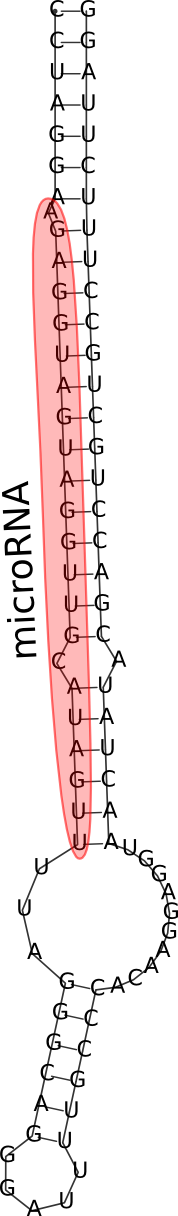
\includegraphics[width=0.6\textwidth]{res/premirna.png}
			\end{center}
		\end{column}

		\begin{column}{0.9\textwidth}
			\begin{itemize}
				\item MicroRNAs (miRNAs) play an essential role in post-transcriptional gene regulation. \pause
					\vspace{10pt}
				\item Precursors of miRNA (pre-miRNAs) are characterized by hairpins structure. \pause
					\vspace{10pt}
				\item A large amount of similar sequences can be folded into this kind of structure. \pause
					\vspace{10pt}
				\item Machine learning algorithms have been proposed to predict which sequences are likely to contain a miRNA.
			\end{itemize}
		\end{column}
	\end{columns}
}

\frame{
	\frametitle{But, there are some problems with ML methods}
	\begin{columns}
		\begin{column}{0.15\textwidth}
			\begin{center}
				
\includegraphics[width=\textwidth]{res/lupa.png}
			\end{center}
		\end{column}

		\begin{column}{0.9\textwidth}
			\begin{itemize}
				\item Datasets used are not representative of the wide variety of negative examples. \\
					$\rightarrow$ Use all hairpins of the genome for validation.
					\pause \vspace{10pt}
				\item The performance measures used underestimate the effect of imbalance. \\
					$\rightarrow$ Take into account the number of false positives.
					\pause \vspace{10pt}
				\item The validation methodology does not imitate a real prediction task. \\
					$\rightarrow$ Test on sequences from unseen species.
					\pause
			\end{itemize}
			\vspace{10pt}
			\centering
			\emph{Taking into account these points, simple sequence alignment works better than machine learning methods.}
		\end{column}
	\end{columns}
}

\subsection{Motivation}
\frame{\frametitle{Can it be done better?}
	\includegraphics<1>[width=\textwidth]{res/better1.pdf}%
	\includegraphics<2>[width=\textwidth]{res/better2.pdf}%
	\includegraphics<3>[width=\textwidth]{res/better3.pdf}%
	\includegraphics<4>[width=\textwidth]{res/better4.pdf}
}


  \section{Proposed method}
  \frame{\tableofcontents[currentsection]}

  \subsection{Convolutional Neural Networks}

\frame{
	\frametitle{A gentle introduction to Convolutional Neural Networks}
	\includegraphics<1-3>[width=\textwidth]{res/cnn_animation0.pdf}%
	\framezoom<2><3>[border=2](0cm,0cm)(3cm,3cm)
	\includegraphics<4>[width=\textwidth]{res/cnn_animation1.pdf}%
	\includegraphics<5>[width=\textwidth]{res/cnn_animation1b.pdf}%
	\includegraphics<6>[width=\textwidth]{res/cnn_animation2.pdf}%
	\includegraphics<7>[width=\textwidth]{res/cnn_animation3.pdf}%
	\includegraphics<8>[width=\textwidth]{res/cnn_animation4.pdf}%
	\includegraphics<9>[width=\textwidth]{res/cnn_animation5.pdf}%
	\includegraphics<10>[width=\textwidth]{res/cnn_animation6.pdf}%
	\includegraphics<11>[width=\textwidth]{res/cnn_animation7.pdf}%
	\includegraphics<12>[width=\textwidth]{res/cnn_animation8.pdf}
}

\subsection{Proposed architecture}
\frame{
	\frametitle{Proposed architecture: mirDNN}
	\includegraphics<1>[width=\textwidth]{res/arquitectura0.pdf}%
	\includegraphics<2>[width=\textwidth]{res/arquitectura1.pdf}%
	\includegraphics<3>[width=\textwidth]{res/arquitectura2.pdf}%
	\includegraphics<4>[width=\textwidth]{res/arquitectura3.pdf}%
	\includegraphics<5>[width=\textwidth]{res/arquitectura4.pdf}%
	\includegraphics<6-7>[width=\textwidth]{res/arquitectura5.pdf}
	\framezoom<6><7>[border=0](6.9cm,3.4cm)(4cm,2.6cm)
}



  \section{Results}
  \frame{\tableofcontents[currentsection]}

  \subsection{Experimental setup}

\frame{\frametitle{Experimental setup}
	\centering
	Validation on a \textit{leave-species-out} scheme \\ \vspace{8pt}
	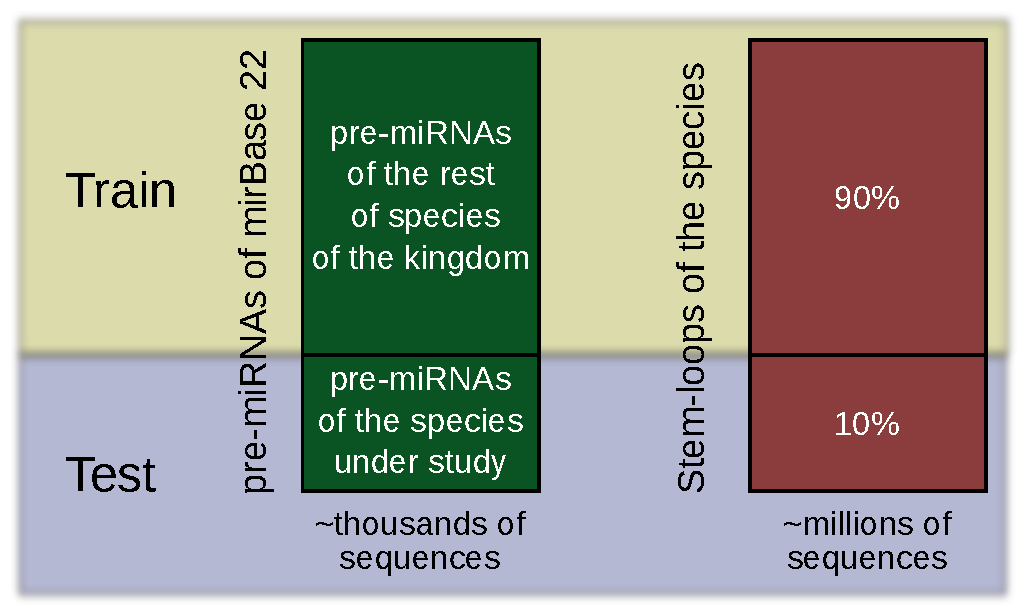
\includegraphics[width=\textwidth]{res/partitions.pdf}
}


\frame{\frametitle{Experimental setup}
\begin{itemize}
	\item Test on three well-known species: \textit{Arabidopsis thaliana}, \textit{Caenorhabditis elegans} and \textit{Anopheles gambiae}. \vspace{8pt} \pause
	\item Two machine learning methods and one sequence alignment method were used for comparison. \vspace{8pt} \pause
	\item The precision and recall were used as performance measures: \vspace{8pt} \\
		\begin{center}
			$Pr = \frac{TP}{TP+FP}$ \hspace{8pt} $Rc = \frac{TP}{TP+FN}$ \vspace{8pt}
		\end{center} \pause
	\item Varying the threshold that defines what is classified as positive or negative, precision-recall curves were generated.
\end{itemize}
}

\subsection{Precision-recall curves}

\frame{\frametitle{Precision-recall curves}
\includegraphics<1>[width=\textwidth]{res/PRROC-ath1.pdf}%
\includegraphics<2>[width=\textwidth]{res/PRROC-ath2.pdf}%
\includegraphics<3>[width=\textwidth]{res/PRROC-cel.pdf}%
\includegraphics<4>[width=\textwidth]{res/PRROC-aga.pdf}
}

\frame{\frametitle{Area under the curves}
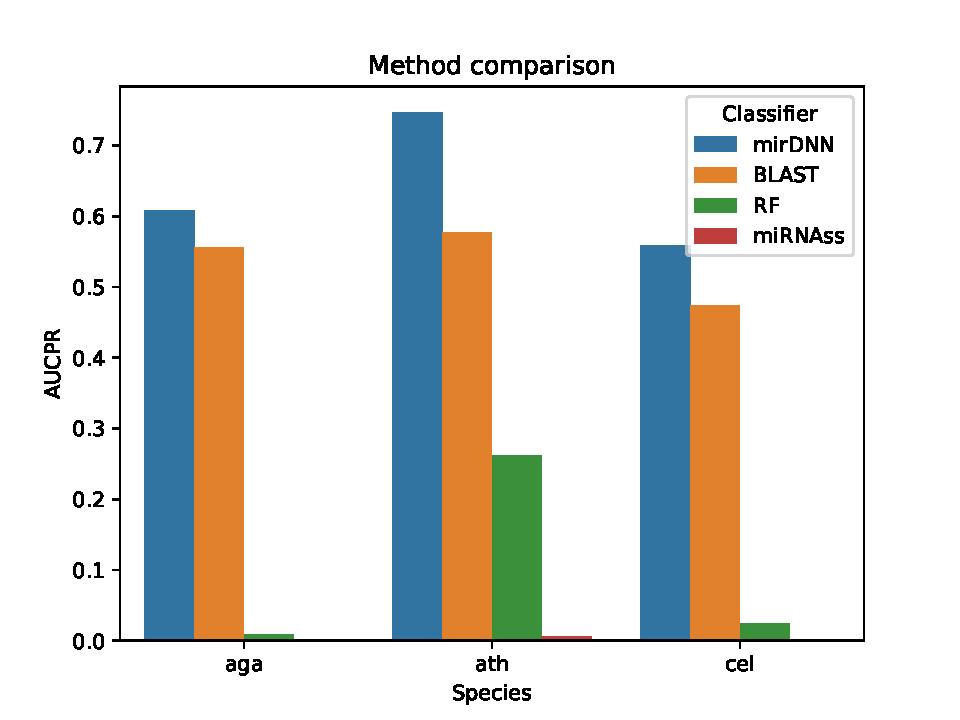
\includegraphics[width=\textwidth]{res/barplot.pdf}
}



  \section{Conclusions}
  \frame{\tableofcontents[currentsection]}

  
\frame{
	\frametitle{Conclusions}
	\begin{itemize}
		\item State-of-the-art machine learning methods for miRNA prediction do not perform well on new species. \pause \vspace{16pt}
		\item Sequence alignment methods have a better performance, but only for low recall rates. \pause \vspace{16pt}
		\item Using convolutional neural networks, we can \textit{learn} which are the important characteristics that define
			a pre-miRNA. \pause \vspace{16pt}
		\item The proposed method achieves a precision many times higher at high recall rates in three tested species.
	\end{itemize}
}


  \frame[plain]{
    \titlepage
    \centering
    \scriptsize \url{cyones@sinc.unl.edu.ar} \\
    \url{http://www.sinc.unl.edu.ar/}
  }

\end{document}
